\section{Problem 3}

\subsection{Problem 3 (a)}

%%%%%%%%%%%%%%% Section 3a :: begins %%%%%%%%%%%%%%%%%%%%
	Intuitively an example of a simple polygon $P$ (with top facet $f$) not castable with translation but castable with only rotation should look like a crescent moon. \Cref{fig:moon} shows the example of such a polygon. As clear from the picture the polygon cannot be casted out with translation only since edge $e$ cannot be pushed against the edge of the mould restricting any translational movements in the upper $180\degree$ arc. Also, if we rotate clockwise taking center $r$, it can be casted out with rotation only. 
	
	
	\begin{figure}[!htbp]
	%	\captionsetup[subfigure]{justification=centering}
		\hspace{-15pt}
		%\begin{subfigure}[b]{1\textwidth}
			\centering
			\resizebox{!}{3cm}{
				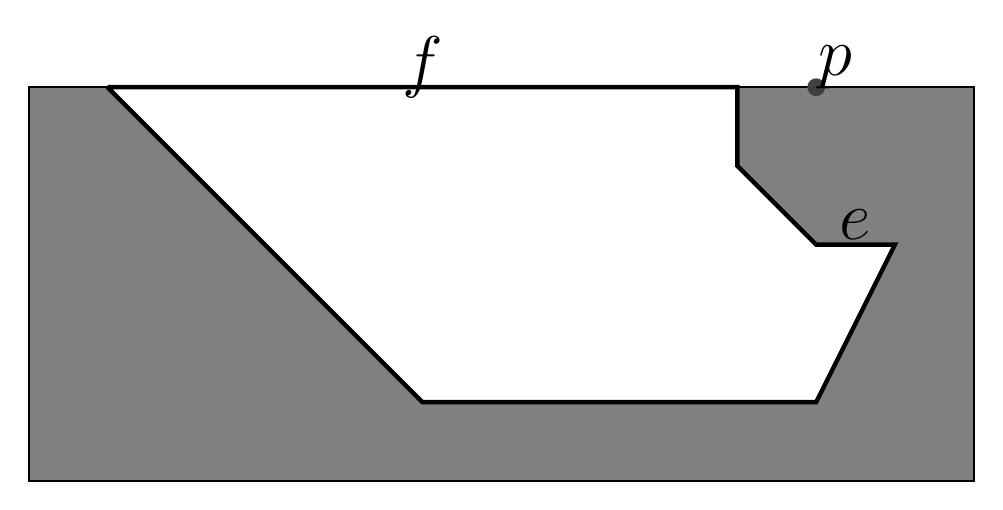
\begin{tikzpicture}
				
				%box
	
				\draw[thick, fill = gray] (-1,-1)rectangle(11,4);
				
				\draw[ultra thick, fill = white] (0,4)--(8,4)--(8,3)--(9,2)--(10,2)--(9,0)--(4,0)--(0,4);
				\filldraw [darkgray] (9,4) circle (3pt);
	
				\draw (9.25,4.25) node {\Huge \textbf{$p$}};
				\draw (9.5,2.25) node {\Huge \textbf{$e$}};
				\draw (4,4.25) node {\Huge \textbf{$f$}};
				\end{tikzpicture}}
			\caption{A simple polygon $P$ (with top facet $f$) not castable with translation but castable with only rotation. $P$ cannot be casted out with translation only since edge $e$ cannot be pushed against the edge of the mould restricting any translational movements in the upper $180\degree$ arc. We rotate clockwise taking center $r$, casting out with rotation only. }
			\label{fig:moon}
		%\end{subfigure}
	\end{figure}
	
	Let's define \textbf{Castable Rotation} as a feasible rotation direction (clockwise or counter clockwise) along with the center of rotation along which the polygon can be casted out of the mold. Depending on the direction of rotation, we define two algorithms for finding out a feasible castable rotation. For the sake of simplicity we just define the algorithm for computing a castable rotation (if any) in clockwise direction, an analogous procedure can be defined for the other orientation of rotation as well.
	
	We list two \textbf{range of motions} possible for nay point along an edge/boundary of $P$:
	\begin{enumerate}
		\item From dynamics of circular motion we know that every point on an edge, say $g$, will be moving perpendicular to the line connecting the center of rotation, say $r$, and the point. This means in the case when we are looking for a castable rotation in clockwise direction, all points along the edge have freedom to move along only the halfplane defined by perpendicular on the edge through the point. Now a plausible movement for the edge can be cosidered only in the region of intersection of all the halfplanes on all points along the considered edge. This \textbf{halfplane is bounded by the line perpendicular to the first vertex} of the edge which we encounter while traversing the boundary of P in clockwise order. In other words, this region defines a halfplane where the center of the clockwise rotation of P can be with respect to the considered edge, so that when the rotation starts no part of the edge would run into the wall of the mold which coincides with e. 
		\item Also, since the mold acts as a  constraint to the motion of and edge, any point along $g$ has freedom only to move along the half plane inwards (opposite to that of the mold).
	\end{enumerate}
	
	For each edge $g$ of $P$, we consider the \textbf{halfplane bounded by the line perpendicular to the first vertex} of $g$ which we encounter while traversing the boundary of $P$ in clockwise order. A feasible region for $r$ to exist can now be computed as a  common intersection of these half-planes corresponding to each of the by $P$'s edges. Hence, the problem reduces to finding the \textbf{intersection of the $n$ halfplanes} which correspond to the $n$ sides of $P$.  As discussed in the lectures, similar to castability of a simple polyhedron, we use a LP to solve our problem in $\bm{O(n)}$ \textbf{expected time} (worst case $\bm{O(nlogn)})$, using \textbf{worst-case} $\bm{O(n)}$ \textbf{storage}. 
	Another (intuitive) way of computing $r$ can be done reducing the number of candidates for being top edges to only a constant number, by considering only segments which lie on the convex hull of $P$ and where at least one adjacent corner of the convex hull is of no more than $90 \degree$. This leaves us with an overall complexity of $O(nlogn)$ time.


	\subsection{Problem 3 (b)}

		%%%%%%%%%%%%%%% Section 3b:: begins %%%%%%%%%%%%%%%%%%%%
		\begin{theorem}
			The closest pair of points in a set $S$ of $n$ points in a plane must be connected by an 
			edge in the Delaunay triangulation of $S$. 
		\end{theorem}
		\begin{proof}
		Consider the Voronoi diagram of $S$, say $vorr(S)$. We approach the proof by means of contradiction. Let us assume that there exists a pair of closest points $p$, $q$ such that the points are not connected by an edge in the Delaunay triangulation. W.l.o.g we can assume that there exists no other point other than $p$ closest to $q$ (analogous statement for $p$). Now consider the circle $C_{pq}$ with diameter as line segment $pq$. From our assumptions we know that no point lies inside as well on the  boundary of circle $C_{pq}$ (although it should be emphasized that this proof can be concluded with out the assumption that there is no point $C_{pq}$ other than $p$, $q$ as points on the circle do not make any difference in arguments, but the assumption is done just for the sake of convenience). Otherwise if there were points on inside the circle then $p$ and $q$ would not be closest pair of points. The center of $C_{pq}$ is equidistant from $p$ as well as $q$, implying that it should be a Voronoi edge common to the faces of cells of $p$ and $q$ in $vorr(S)$. This implies that $(p,q)$ is an edge in the Delaunay triangulation which gives a contradiction to our initial assumption. This concludes the proof.		
		\end{proof}

		%%%%%%%%%%%%%%% Section 3b:: ends %%%%%%%%%%%%%%%%%%%%